\subsection{Corrected-source learning curves}

The corrected annotation protocol produced agreement on 5,979 of 9,077 candidates;
3,098 still require review. These are agreements between models, with no
independent human labels. Finalization removed seven repeated or cross-partition
candidate copies, leaving 5,548 training rows and 424 development rows. The
conservative source graph places the training rows in one connected component
and the development rows in thirty components. Of the development rows, 66
belong to previously examined components and 358 to newly allocated development
components. Both slices are development data. Reserved confirmation records
were not read or fitted.

Training retention labels comprise 233 durable, 4,522 temporary, 517 ignore,
and 276 uncertain examples. Development contains 14, 346, 40, and 24 examples
respectively. Of 360 typed development examples, 304 are projects, 31 facts,
24 preferences, and one a routine; behavior and relationship have no support.
The training sources therefore expand volume much more than class diversity.
Agreement filtering and conservative source quarantine can also change the
distribution being measured.

We fitted multinomial logistic heads over a frozen MiniLM encoder at five
natural-source counts: 0, 100, 500, 2,000, and all 3,332 source units. All fits
retain 1,063 original synthetic training examples. Three seeded, nested
source-prefix draws define the intermediate points. Each identical zero-source
and full-source endpoint is fitted once per weighting rule. Unweighted and
inverse-frequency class-balanced fitting yield 22 pairs of heads. The heads
use $C=10$ and at most 1,500 optimizer iterations; every fit converged before
that limit. Candidate context matches the serving contract. All formatted inputs fit its
declared 256-token limit, with no silent truncation.

Temperature is selected separately for each head by development negative
log-likelihood from $\{0.5,0.75,1,1.5,2,3,5\}$. Reporting selective performance
on that same set makes the calibration results optimistic. The fixed joint
acceptance threshold is 0.8. At the full-source endpoints, retention temperature
is 1.5 and type temperature is 1.0 for both weighting rules. Source counts and
fitting costs intentionally vary: this experiment measures data scaling, not
an equal-compute replay advantage.

\begin{figure}[htbp]
\centering
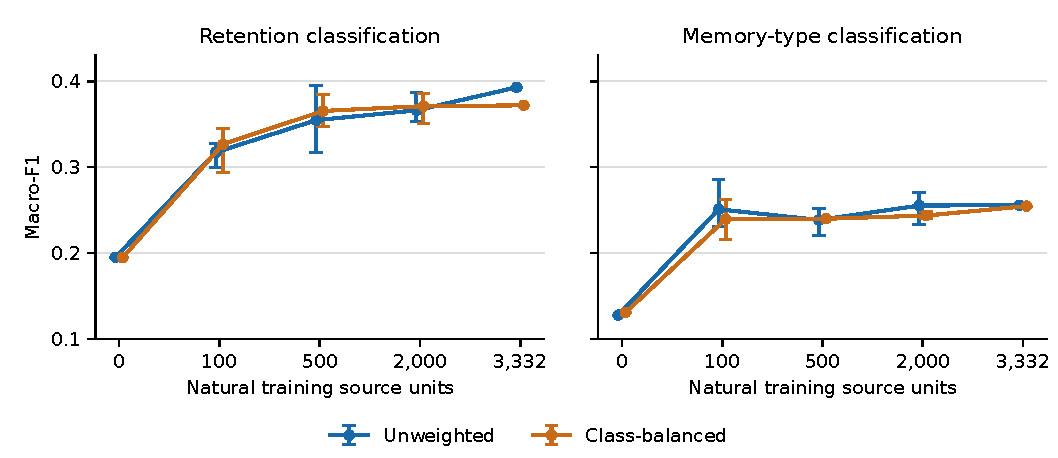
\includegraphics[width=\linewidth]{images/expanded-learning-curves.pdf}
\caption{Development learning curves on provisional labels. Source counts are
shown at equally spaced categorical positions. Points are means and bars are
the ranges of three source-subset draws at intermediate counts, not confidence
intervals. Endpoints contain one fit per weighting rule. Type macro-F1 averages
all six configured classes, assigning zero F1 to the two classes with no
development support; their recall remains unevaluated.}
\label{fig:expanded-curves}
\end{figure}

Unweighted retention macro-F1 increases from 0.195 with synthetic examples
alone to 0.393 at the full-source endpoint (Figure~\ref{fig:expanded-curves}).
That endpoint recovers none of the fourteen durable examples. Class balancing
recovers five, but predicts durable for seventy examples, of which sixty-five
disagree with the provisional labels. Its durable precision is therefore
$5/70=7.1\%$. Higher aggregate agreement does not establish useful durable-memory
admission.

\begin{table}[htbp]
\centering\small
\begin{tabular}{lrrrr}
\toprule
Training rule & Retention F1 & Type F1 & Durable hits & Joint errors/accepted\\
\midrule
Training majority & 0.225 & 0.153 & 0/14 & ---\\
Unweighted & 0.393 & 0.256 & 0/14 & 14/151\\
Class-balanced & 0.372 & 0.255 & 5/14 & 7/28\\
\bottomrule
\end{tabular}
\caption{Full-source development results. F1 is macro-averaged over four
retention or six type classes. The majority labels are selected from training
data only. Joint errors are disagreements with provisional labels among
accepted predictions, with coverage denominators of 424. They are neither
independently reviewed errors nor unsupported-memory counts.}
\label{tab:expanded-classification}
\end{table}

At threshold 0.8, unweighted fitting accepts 151/424 examples (35.6\%) with
14/151 disagreements (9.3\%). Balanced fitting accepts 28/424 (6.6\%) with
7/28 disagreements (25.0\%). The training-majority retention prediction alone
has 81.6\% accuracy, compared with 80.7\% unweighted and 61.3\% balanced
accuracy. Project dominance similarly makes majority type accuracy 84.4\%.
Accuracy therefore obscures substantial minority-class failures.

Encoding 7,035 rows required 384,356 input tokens, 16.1 seconds wall time and
29.1 CPU seconds on the shared local machine. The 22 head fits and their reports
took a summed 2.5 seconds wall time and 2.5 CPU seconds. These totals exclude
source extraction, annotation, model loading, and earlier synthetic generation.
They are not an isolated throughput benchmark. Per-class confusion matrices,
calibration diagnostics, source-subset ranges, and both development slices
accompany the paper as aggregate data.

No classifier is promoted from this comparison. The next development study
should test representation adaptation and loss weighting against these frozen
baselines, while improving independently reviewed class coverage. Increasing
the same source distribution alone does not resolve the observed durable-class
failure or establish a sleep-inspired learning benefit.
